\documentclass[crop]{standalone}

\usepackage{../../../supplementary/header/header_pgfplot_standalone}

\pgfplotsset{compat=newest,
			xtick pos=left,
			ytick pos=left
			}
			

\begin{document}
\begin{tikzpicture}

\begin{axis}[
	height=230pt,
	width=418pt,
%Type
	bar width=15pt,
	%nodes near coords,
	axis on top,
	enlarge x limits=0.04,
	symbolic x coords={vfe,iqe,droop,lee,ce-red,ce-green,se,pce},
%Domain
	ymin=0,ymax=110,
	xmin=vfe,xmax=pce,
%Axis Labels
    xticklabel style={align=center},
    yticklabels={,0,20,40,60,80,100},
	ylabel=Efficiency \text{[}\%\text{]},
	xticklabels={,V$_\text{f}$E, IQE, Droop, LEE, CE \\ (\textcolor{red}{Red}), CE \\ (\textcolor{teal}{Green}/\textcolor{orange}{black}), SE, \textbf{PCE}},
%Legend
    legend style={at={(0.12,0.02)},anchor=south west},
	legend cell align={left},
	legend style={draw=none,fill=none},
	%nodes near coords,
			]
\addlegendimage{/pgfplots/refstyle=bluebar}
\addlegendentry{Spillover}
\addlegendimage{/pgfplots/refstyle=graybar}
\addlegendentry{Other Improvements}
]
%Hidden bar to push other bars to 2003 level
\addplot [ybar stacked,fill=none,draw=none]
	table [col sep=comma, x=losschannel, y=hiddenbar]
	{../data/efficiency_breakthroughs.csv};
%1 OTHER
\addplot [ybar stacked,fill=gray!30,draw=gray]
	table [col sep=comma, x=losschannel, y=o-1]
	{../data/efficiency_breakthroughs.csv}; \label{graybar}
%1 OTHER
\addplot [ybar stacked,fill=blue!30,draw=blue]
	table [col sep=comma, x=losschannel, y=so-1]
	{../data/efficiency_breakthroughs.csv}; \label{bluebar}.
%2 OTHER
\addplot [ybar stacked,fill=gray!30,draw=gray]
	table [col sep=comma, x=losschannel, y=o-2]
	{../data/efficiency_breakthroughs.csv}; \label{graybar}
%2 OTHER
\addplot [ybar stacked,fill=blue!30,draw=blue]
	table [col sep=comma, x=losschannel, y=so-2]
	{../data/efficiency_breakthroughs.csv}; \label{bluebar}
%1 OTHER
\addplot [ybar stacked,fill=gray!30,draw=gray]
	table [col sep=comma, x=losschannel, y=o-3]
	{../data/efficiency_breakthroughs.csv}; \label{graybar}
%1 OTHER
\addplot [ybar stacked,fill=blue!30,draw=blue]
	table [col sep=comma, x=losschannel, y=so-3]
	{../data/efficiency_breakthroughs.csv}; \label{bluebar}
\end{axis}

%Years Legend only
\begin{axis}[
	height=230pt,
	width=418pt,
%Type
	%nodes near coords,
	axis on top,
	enlarge x limits=0.04,
%Domain
	ymin=0,ymax=110,
	xmin=0,xmax=7,
%Axis Labels
	%ylabel=Efficiency \text{[}\%\text{]},
	yticklabels={,,},
	xticklabels={,,},
%Legend
    legend style={at={(0.65,0.02)},anchor=south west},
	legend cell align={left},
	legend style={draw=none,fill=none},
			]
\addlegendimage{no markers, thick, purple}
\addlegendentry{2020}
\addlegendimage{no markers, thick, magenta}
\addlegendentry{2016}
\addlegendimage{no markers, thick, orange}
\addlegendentry{2010}
\addlegendimage{no markers, thick, teal}
\addlegendentry{2002}
\addlegendimage{no markers, thick, blue}
\addlegendentry{1997}
\addlegendimage{no markers, thick, black}
\addlegendentry{Physical Limit}
]
%Table
\node [above right] at (rel axis cs:0.4,0.03) {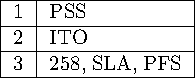
\includegraphics[width=83pt]{table.pdf}};
%Annotations
%VfE
\node [] at (0,65) {\textcolor{teal}{N/A}};
%CE
\node [] at (6.35,73.5) {3};
%Droop
\node [] at (2,60) {\textcolor{teal}{N/A}};
%LEE
\node [] at (3.35,45) {2};
\node [] at (3.35,68) {1};
%CE (Red)
\node [] at (4,40) {\textcolor{teal}{N/A}};
%CE (Green)
\node [] at (5,56) {\textcolor{teal}{N/A}};
%SE
\node [] at (6,64) {\textcolor{teal}{N/A}};
%Efficiency Lines per Year
%VfE
\draw [teal, thick] (axis cs:-0.25,70) -- (axis cs:0.25,70);
\draw [orange, thick] (axis cs:-0.25,85) -- (axis cs:0.25,85);
\draw [magenta, thick] (axis cs:-0.25,96) -- (axis cs:0.25,96);
\draw [purple, thick] (axis cs:-0.25,99.5) -- (axis cs:0.25,99.5);
\draw[->, black, thick] (axis cs:0,103) -- (axis cs:0,107);
%IQE
\draw [blue, thick] (axis cs:0.75,40) -- (axis cs:1.25,40);
\draw [teal, thick] (axis cs:0.75,55) -- (axis cs:1.25,55);
\draw [orange, thick] (axis cs:0.75,70) -- (axis cs:1.25,70);
\draw [magenta, thick] (axis cs:0.75,88.02) -- (axis cs:1.25,88.02);
\draw [purple, thick] (axis cs:0.75,90) -- (axis cs:1.25,90);
\draw [black, thick] (axis cs:0.75,100) -- (axis cs:1.25,100);
%Droop
\draw [teal, thick] (axis cs:1.75,65) -- (axis cs:2.25,65);
\draw [orange, thick] (axis cs:1.75,70) -- (axis cs:2.25,70);
\draw [magenta, thick] (axis cs:1.75,89.06) -- (axis cs:2.25,89.06);
\draw [purple, thick] (axis cs:1.75,90.06) -- (axis cs:2.25,90.06);
\draw [black, thick] (axis cs:1.75,100) -- (axis cs:2.25,100);
%LEE
\draw [blue, thick] (axis cs:2.75,30) -- (axis cs:3.25,30);
\draw [teal, thick] (axis cs:2.75,60) -- (axis cs:3.25,60);
\draw [orange, thick] (axis cs:2.75,80) -- (axis cs:3.25,80);
\draw [magenta, thick] (axis cs:2.75,86.86) -- (axis cs:3.25,86.86);
\draw [purple, thick] (axis cs:2.75,90) -- (axis cs:3.25,90);
\draw [black, thick] (axis cs:2.75,100) -- (axis cs:3.25,100);
%CE(Red)
\draw [teal, thick] (axis cs:3.75,45.265) -- (axis cs:4.25,45.265);
\draw [orange, thick] (axis cs:3.75,51.12) -- (axis cs:4.25,51.12);
\draw [magenta, thick] (axis cs:3.75,51.12) -- (axis cs:4.25,51.12);
\draw [purple, thick] (axis cs:3.75,56) -- (axis cs:4.25,56);
\draw [black, thick] (axis cs:3.75,70) -- (axis cs:4.25,70);
%CE(Green/black)
\draw [teal, thick] (axis cs:4.75,65) -- (axis cs:5.25,65);
\draw [orange, thick] (axis cs:4.75,61) -- (axis cs:5.25,61);
\draw [magenta, thick] (axis cs:4.75,79.32398267) -- (axis cs:5.25,79.32398267);
\draw [purple, thick] (axis cs:4.75,80) -- (axis cs:5.25,80);
\draw [black, thick] (axis cs:4.75,91) -- (axis cs:5.25,91);
%SE
\draw [teal, thick] (axis cs:5.75,74) -- (axis cs:6.25,74);
\draw [orange, thick] (axis cs:5.75,69.24939467) -- (axis cs:6.25,69.24939467);
\draw [magenta, thick] (axis cs:5.75,78.17) -- (axis cs:6.25,78.17);
\draw [purple, thick] (axis cs:5.75,83) -- (axis cs:6.25,83);
\draw [black, thick] (axis cs:5.75,100) -- (axis cs:6.25,100);
\end{axis}

\end{tikzpicture}
\end{document}
